\documentclass[tikz,border=10pt]{standalone}
\usepackage{fontspec}
\setmainfont{Arial}
\usetikzlibrary{shapes,arrows.meta,positioning,fit,calc}

\definecolor{navy}{RGB}{20, 45, 80}
\definecolor{barrierred}{RGB}{185, 28, 28}
\definecolor{paperbg}{RGB}{250, 252, 255}
\definecolor{paperborder}{RGB}{147, 197, 253}
\definecolor{shelfbg}{RGB}{248, 250, 252}
\definecolor{shelfborder}{RGB}{203, 213, 225}

\begin{document}
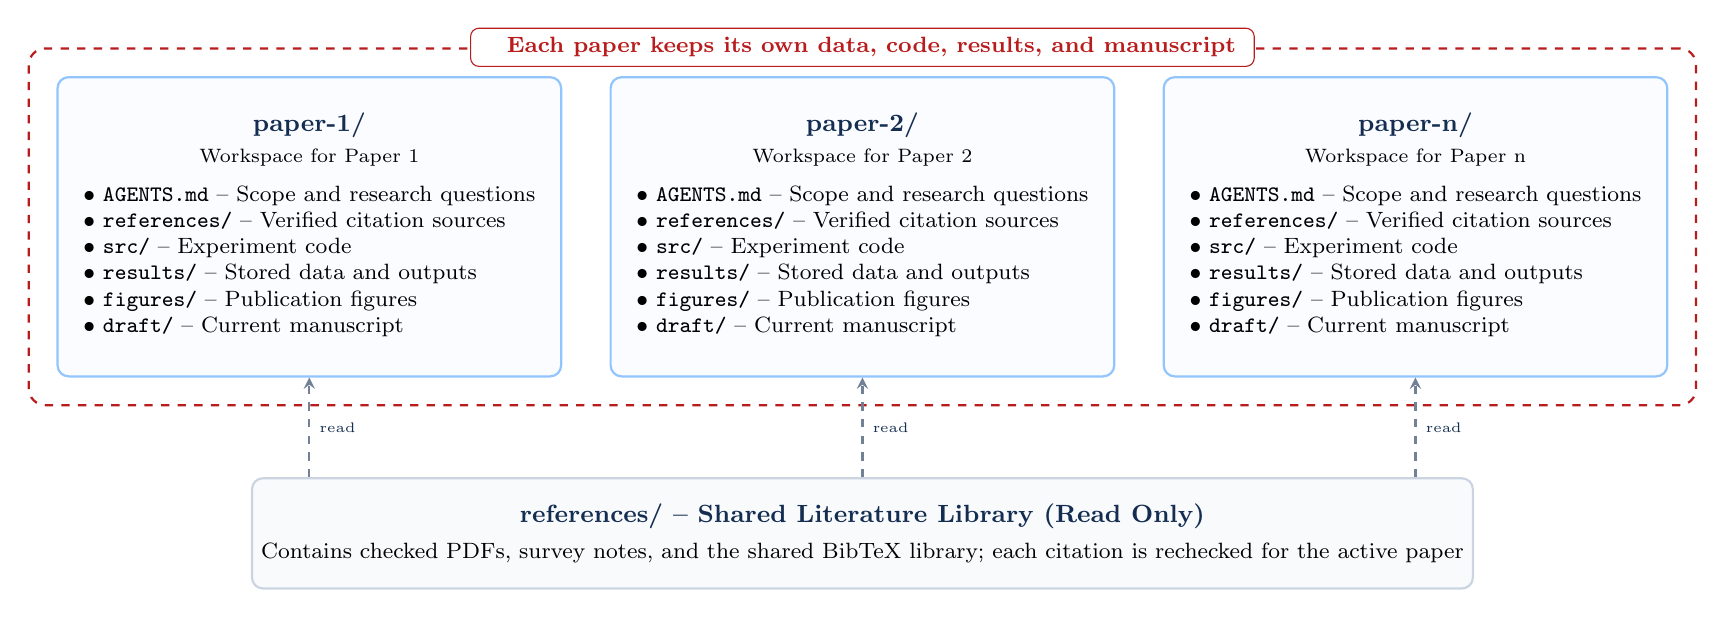
\begin{tikzpicture}[
  >=stealth,
  node distance=0.8cm and 0.6cm,
  paper/.style={
    draw=paperborder,
    fill=paperbg,
    rounded corners=4pt,
    thick,
    minimum width=4.3cm,
    minimum height=3.8cm,
    align=center,
    font=\small
  },
  shelf/.style={
    draw=shelfborder,
    fill=shelfbg,
    rounded corners=4pt,
    thick,
    minimum width=14.4cm,
    minimum height=1.4cm,
    align=center,
    font=\small
  }
]

  % 3 Generic Paper Workspaces
  \node[paper] (p1) {
    \textbf{\textcolor{navy}{paper-1/}}\\\scriptsize Workspace for Paper 1\\[5pt]
    \footnotesize
    \begin{tabular}{l}
      $\bullet$ \texttt{AGENTS.md} -- Scope and research questions\\
      $\bullet$ \texttt{references/} -- Verified citation sources\\
      $\bullet$ \texttt{src/} -- Experiment code\\
      $\bullet$ \texttt{results/} -- Stored data and outputs\\
      $\bullet$ \texttt{figures/} -- Publication figures\\
      $\bullet$ \texttt{draft/} -- Current manuscript
    \end{tabular}
  };

  \node[paper, right=of p1] (p2) {
    \textbf{\textcolor{navy}{paper-2/}}\\\scriptsize Workspace for Paper 2\\[5pt]
    \footnotesize
    \begin{tabular}{l}
      $\bullet$ \texttt{AGENTS.md} -- Scope and research questions\\
      $\bullet$ \texttt{references/} -- Verified citation sources\\
      $\bullet$ \texttt{src/} -- Experiment code\\
      $\bullet$ \texttt{results/} -- Stored data and outputs\\
      $\bullet$ \texttt{figures/} -- Publication figures\\
      $\bullet$ \texttt{draft/} -- Current manuscript
    \end{tabular}
  };

  \node[paper, right=of p2] (p3) {
    \textbf{\textcolor{navy}{paper-n/}}\\\scriptsize Workspace for Paper n\\[5pt]
    \footnotesize
    \begin{tabular}{l}
      $\bullet$ \texttt{AGENTS.md} -- Scope and research questions\\
      $\bullet$ \texttt{references/} -- Verified citation sources\\
      $\bullet$ \texttt{src/} -- Experiment code\\
      $\bullet$ \texttt{results/} -- Stored data and outputs\\
      $\bullet$ \texttt{figures/} -- Publication figures\\
      $\bullet$ \texttt{draft/} -- Current manuscript
    \end{tabular}
  };

  % Barrier Box
  \node[draw=barrierred, dashed, thick, rounded corners=6pt, inner sep=10pt, fit=(p1) (p2) (p3)] (barrier) {};
  \node[fill=white, draw=barrierred, rounded corners=3pt, font=\footnotesize\bfseries, text=barrierred] at (barrier.north) {\quad Each paper keeps its own data, code, results, and manuscript \quad};

  % Shared Shelf Below
  \node[shelf, below=0.9cm of barrier] (shelf) {
    \textbf{\textcolor{navy}{references/ -- Shared Literature Library (Read Only)}}\\[2pt]
    \footnotesize Contains checked PDFs, survey notes, and the shared BibTeX library; each citation is rechecked for the active paper
  };

  \draw[->, thick, dashed, draw=navy!60] (shelf.north -| p1.south) -- (p1.south) node[midway, right, font=\tiny, text=navy] {read};
  \draw[->, thick, dashed, draw=navy!60] (shelf.north -| p2.south) -- (p2.south) node[midway, right, font=\tiny, text=navy] {read};
  \draw[->, thick, dashed, draw=navy!60] (shelf.north -| p3.south) -- (p3.south) node[midway, right, font=\tiny, text=navy] {read};

\end{tikzpicture}
\end{document}
